\section{Exploratory analysis: removing the upstream risk score}\label{sec:ablation}

\textbf{Why this extension matters.} The full-input comparison asks whether a readable downstream rule can compete with a boosted-tree ensemble on the same information. It does not establish an entirely interpretable credit-assessment process: \var{ExternalRiskEstimate} is itself a consolidated score with undocumented construction in the available material. If much of its predictive work is performed upstream, a simple downstream model can inherit that work without exposing its mechanism. This is a substantive qualification of the interpretation of the original experiment, not an accusation that the input is invalid or leaked.

\textbf{Design and status.} After inspecting the main results, we specified a score-removal extension in \texttt{docs/Protocol.md}. It is explicitly exploratory. We remove \var{ExternalRiskEstimate} and its special-state indicator, leaving \NNoScoreVars{} original variables and \NNoScoreCols{} encoded columns. The modelling population and every development, test and inner-CV customer membership remain unchanged. In particular, exclusion of all-$-9$ records is determined from the full records before score removal. Each of the three families is retuned from the same predefined search space using mean CV Brier, including the same training-only early-stopping procedure for XGBoost. Simply deleting the score at prediction time would not be a meaningful comparison, because a trained model expects its original inputs; fixing its original hyperparameters would also disadvantage a model whose optimal complexity changes with its inputs.

\begin{table}[htbp]
\centering\small
\caption{Exploratory score-removal comparison on the same final-test customers. Each no-score model was independently retuned on development folds. The calibration slope is diagnostic and was not used to alter test predictions.}
\label{tab:ablation}
\begin{tabular}{@{}llrrrr@{}}
\toprule
Model & Inputs & AUC & Brier & Log-loss & Cal. slope \\
\midrule
L1 logistic & Full & 0.792 & 0.1856 & 0.554 & 0.95 \\
L1 logistic & No score & 0.791 & 0.1861 & 0.556 & 0.93 \\
CART & Full & 0.758 & 0.2009 & 0.589 & 0.83 \\
CART & No score & 0.754 & 0.2001 & 0.588 & 0.86 \\
XGBoost & Full & 0.796 & 0.1843 & 0.549 & 0.96 \\
XGBoost & No score & 0.794 & 0.1850 & 0.551 & 0.91 \\
\bottomrule
\end{tabular}

\end{table}

\begin{figure}[htbp]
\centering
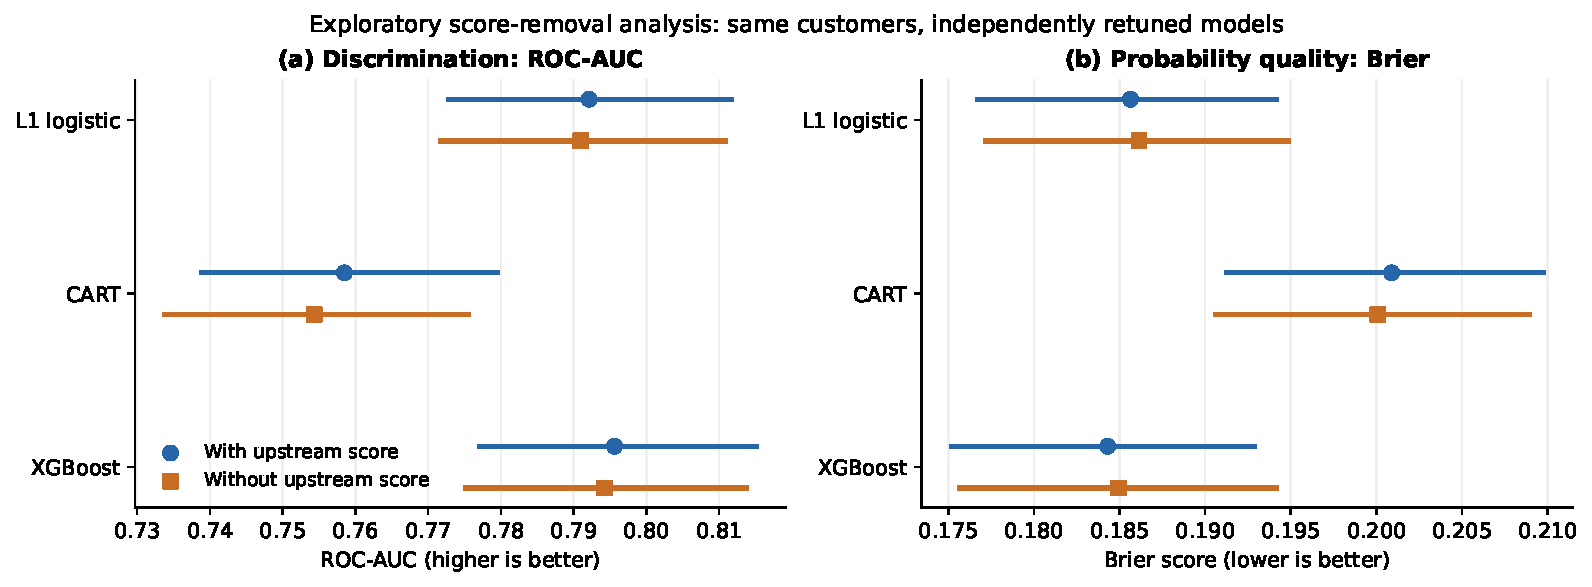
\includegraphics[width=\textwidth]{../results/figures/fig4_ablation_performance.pdf}
\caption{Full versus no-score models. Bars are paired-bootstrap marginal intervals for each model's metric, conditional on its fit. Overlap of these marginal intervals is not the test for a paired difference; see Table~\ref{tab:ablationdiff}.}
\label{fig:ablationperformance}
\end{figure}

\textbf{Aggregate changes.} Without the score, the test AUCs are \NoScoreAUCLR{} for logistic regression, \NoScoreAUCCART{} for CART and \NoScoreAUCXGB{} for XGBoost. The corresponding Brier scores are \NoScoreBrierLR{}, \NoScoreBrierCART{} and \NoScoreBrierXGB{}. Table~\ref{tab:ablationdiff} gives within-family changes using a consistent \emph{full minus no-score} convention: positive AUC changes favour keeping the score, while negative Brier changes favour keeping it. These intervals concern the predictive value of including this input within our learning procedure. They do not estimate a causal effect of the upstream score on default, a benefit of a lending decision, or an intervention on applicants.

\begin{table}[htbp]
\centering\small
\caption{Paired changes from score removal, conditional on the fitted models. Differences are full minus no-score. The comparison is exploratory; no multiplicity-adjusted or equivalence claim is made.}
\label{tab:ablationdiff}
\begin{tabular}{@{}lrr@{}}
\toprule
Model & AUC difference [95\% CI] & Brier difference [95\% CI] \\
\midrule
L1 logistic & \ScoreDeltaAUCLR \ScoreDeltaAUCciLR & \ScoreDeltaBrierLR \ScoreDeltaBrierciLR \\
CART & \ScoreDeltaAUCCART \ScoreDeltaAUCciCART & \ScoreDeltaBrierCART \ScoreDeltaBrierciCART \\
XGBoost & \ScoreDeltaAUCXGB \ScoreDeltaAUCciXGB & \ScoreDeltaBrierXGB \ScoreDeltaBrierciXGB \\
\bottomrule
\end{tabular}

\end{table}

The observed XGBoost-minus-logistic AUC gap is \GapFullXGBLR{} with the score and \GapNoScoreXGBLR{} without it. The observed gap remains small in both settings. This weakens the suggestion that their proximity is \emph{entirely} explained by sharing that one score, but does not show that the score contains no useful information: other bureau variables may substitute for it, and most development splits favour keeping it. All three test AUC-change intervals include zero; this is uncertainty about incremental performance, not a proof of equivalence or a universal property of interpretable models. The no-score logistic model has \NoScoreLRCoef{} non-zero coefficients on \NoScoreLRVars{} original variables; its actual sparsity, rather than the label ``L1'', is what matters for inspection.

\textbf{Development-split evidence.} We repeated the full no-score selection procedure on the same ten development holdouts used for the full-input comparison (Fig.~\ref{fig:ablationrepeated}). Including the score gives a higher AUC in \RepScoreAUCPosLR{} of ten splits for logistic regression, \RepScoreAUCPosCART{} for CART and \RepScoreAUCPosXGB{} for XGBoost. Mean paired AUC changes are \RepScoreAUCMeanLR{}, \RepScoreAUCMeanCART{} and \RepScoreAUCMeanXGB{}, respectively. These are overlapping resamples from one development population. Their spread is a sensitivity description, not a confidence interval based on ten independent studies.

\begin{figure}[htbp]
\centering
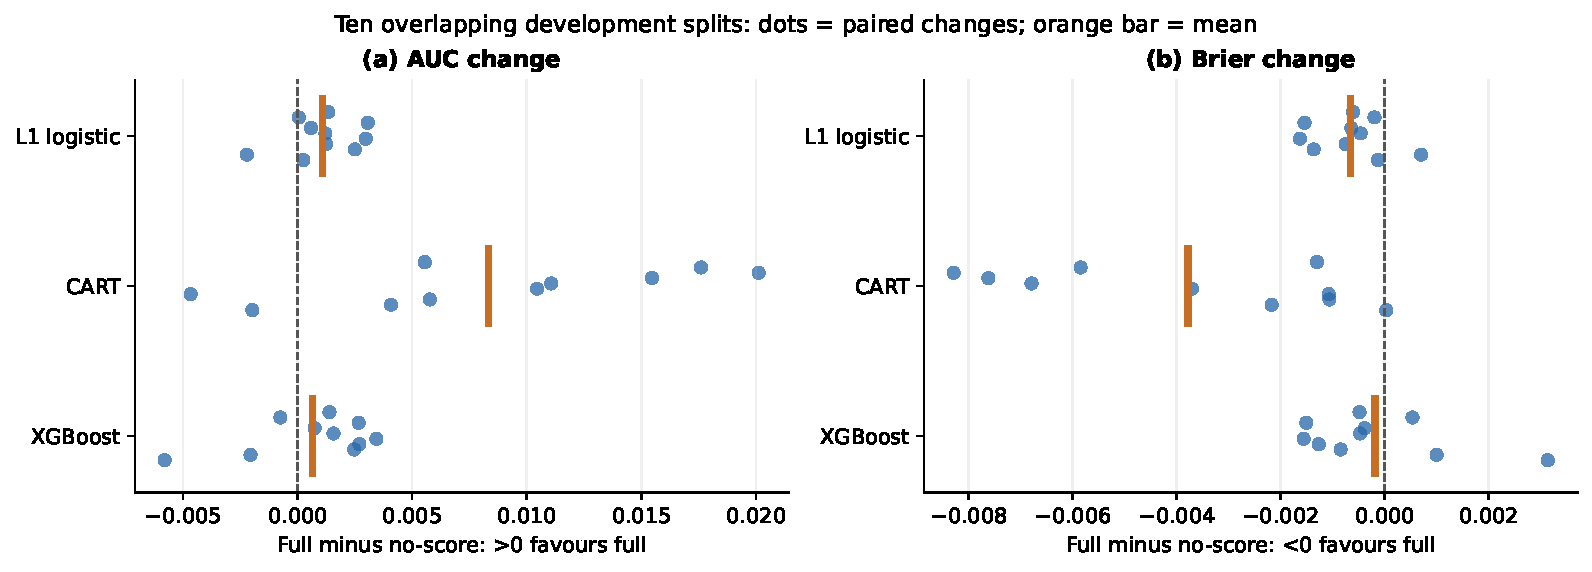
\includegraphics[width=\textwidth]{../results/figures/fig6_ablation_repeated.pdf}
\caption{Effect of score removal within each repeated development split, with both variants retuned on the corresponding training portion. The orange bar is the descriptive mean, not a significance test.}
\label{fig:ablationrepeated}
\end{figure}

\textbf{Individual changes.} Aggregate changes conceal a much larger restructuring of the tree: its AUC change is modest, but nearly half of its customers move by more than 0.10 in predicted risk. This is a comparison of two independently retuned models, not an intervention on one frozen model or on a person. Dropping the score changes predicted default probabilities by more than 0.10 for \NoScoreChangeTenLR{} of test customers under logistic regression, \NoScoreChangeTenCART{} under CART and \NoScoreChangeTenXGB{} under XGBoost (Fig.~\ref{fig:ablationindividual}). Mean absolute changes are \NoScoreMeanChangeLR{}, \NoScoreMeanChangeCART{} and \NoScoreMeanChangeXGB{}. Label disagreement at the descriptive 0.5 threshold is \NoScoreLabelChangeLR{}, \NoScoreLabelChangeCART{} and \NoScoreLabelChangeXGB{}, respectively. Aggregate score changes alone therefore do not describe how the alternative models treat the same recorded applicant. We have no lending-cost model and do not treat 0.5 as an optimal approval threshold.

\begin{figure}[htbp]
\centering
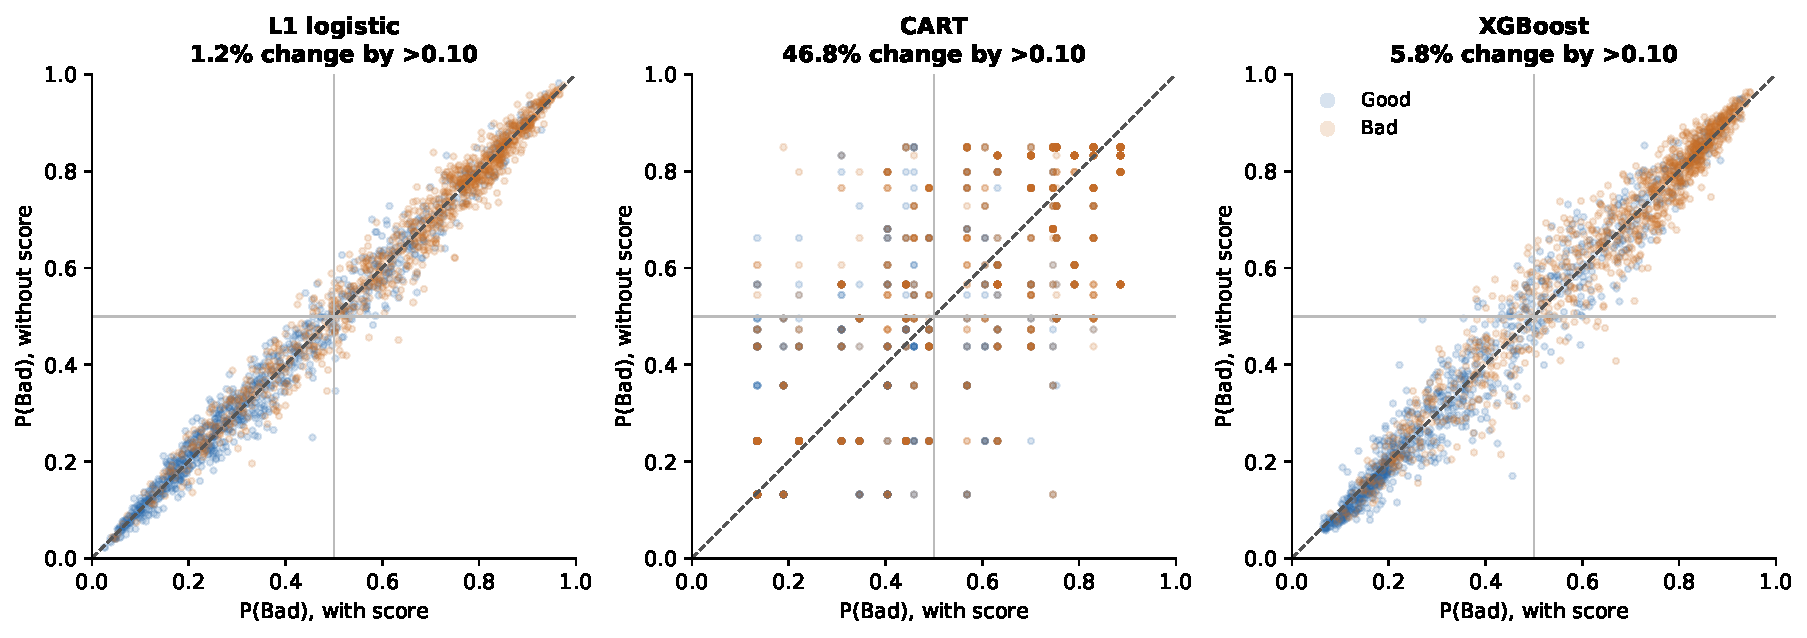
\includegraphics[width=\textwidth]{../results/figures/fig5_ablation_individual.pdf}
\caption{Each point is the same test customer scored by a full and no-score model. Colours denote the observed outcome, not a protected group. Distance from the diagonal indicates a changed probability; crossing a grey line at 0.5 is not evidence of an actual changed lending decision.}
\label{fig:ablationindividual}
\end{figure}

\textbf{Probability validation remains separate.} Figure~\ref{fig:ablationcalibration} shows reliability curves and recalibration slopes for both variants. Brier and log-loss measure overall probability quality, including discrimination and calibration; neither is a pure calibration score. A slope and a binned curve are finite-sample diagnostics, with no formal calibration-equivalence claim. All diagnostics use the models' original predictions, without calibrating them on the test labels.

\begin{figure}[htbp]
\centering
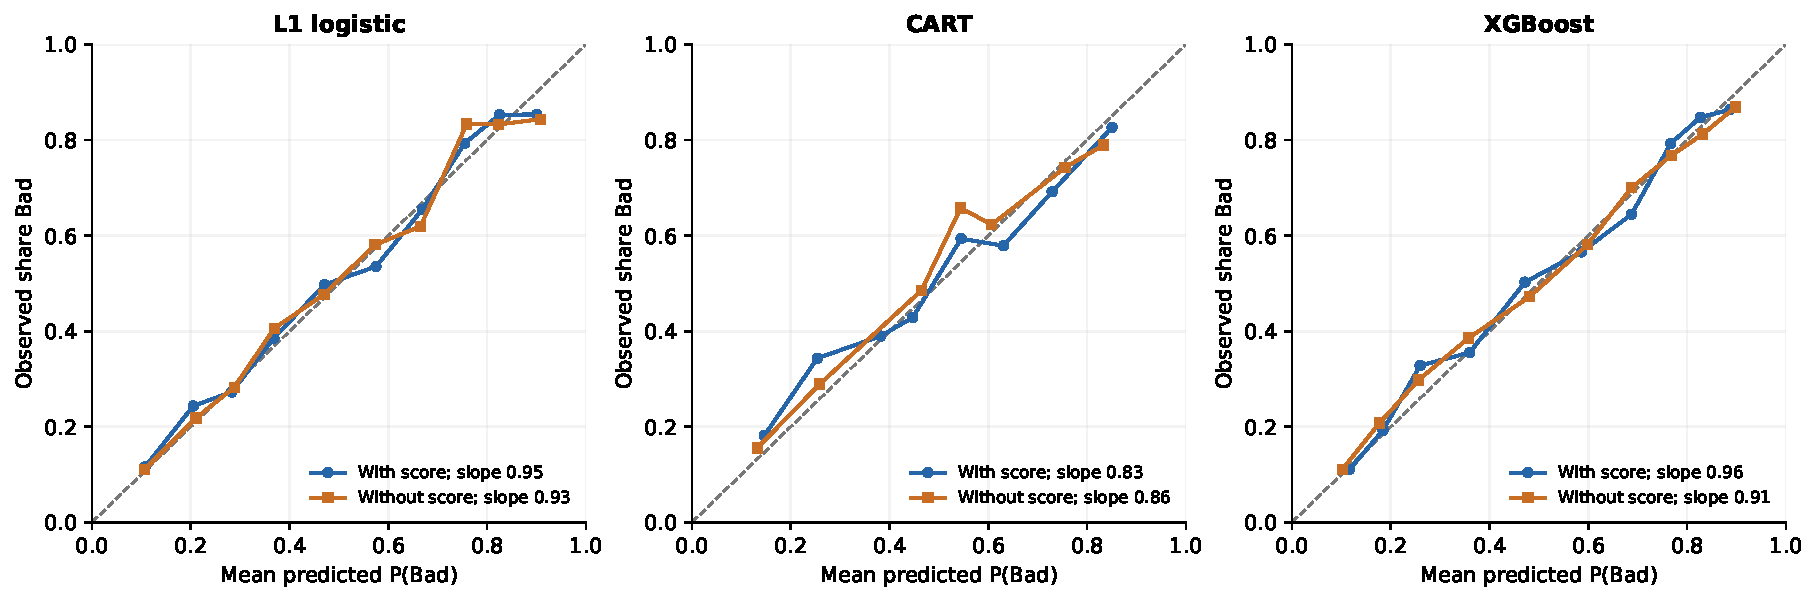
\includegraphics[width=\textwidth]{../results/figures/fig7_ablation_calibration.pdf}
\caption{Calibration diagnostics before and after score removal, using ten quantile bins where distinct predictions permit them. Curves are descriptive estimates on one historical test sample.}
\label{fig:ablationcalibration}
\end{figure}

\textbf{Interpretation limit.} Removing a score cannot remove all information associated with it: the remaining bureau variables may contain overlapping signals, and their own measurement pipeline is only partly documented. The ablation asks about incremental predictive dependence under refitting, not how the upstream score was computed. It also supplies no genuine temporal, institutional or prospective external validation. Thus it sharpens the comparison relevant to Rudin without replacing the validation demanded by Ghassemi et al.
